\textbf{List the formulas you have used to convert GPS coordinates to NED positions and attach your corresponding codes for this step.}\\

To convert from GPS coordinates to NED positions, it is required that you convert from Geodetic coordinate frame $ [longitude ($\lambda$), latitude ($\phi$), altitude (h)]^T$ to Earth-Centered, Earth Fixed (ECEF) coordinate frame $[$x_e$, $y_e$, $z_e$]^T$ to North-East-Down (NED) coordinate frame $[$x_n$, $y_n$, $z_n$]^T$. \\
To Convert from Geodetic to ECEF, you need to define Earth's Equatorial radius (a), Earth's Polar radius (b), which can then be used to calculate the eccentricity of the Earth ellipsoid (e). These variables are used to define the Prime vertical radius of curvature N($\varphi$). The equations shown in Eq.(\ref{Geo2ECEF}) will be used to compute the ECEF coordinates.

\begin{equation}
\begin{aligned}
X_e &= \left(N(\varphi) + h\right) \cos \varphi \cos \lambda\\
Y_e &= \left(N(\varphi) + h\right) \cos \varphi \sin \lambda\\
Z_e &= \left(\frac{b^2}{a^2} N(\varphi) + h \right) \sin \varphi
\end{aligned}
\label{Geo2ECEF}
\end{equation}

where
\begin{equation}
N(\varphi) = \frac{a^2}{\sqrt{a^2 \cos^2 \varphi + b^2 \sin^2 \varphi}} = \frac{a^2}{\sqrt{1 - e^2 \sin^2 \varphi}}
\label{N_phi}
\end{equation} \\

You begin by converting the latitude, and longitude to radians, since they are provided to us in degrees. The size of the latitude, longitude, altitude, and time vectors are 10215 x 1, so the converted latitude and longitude in radians will also be a 10215 x 1 vector. The first step now will be to define the initial UAV position as the reference position being used for the coordinate transformation. This initial position will be the first input in the data set at time index = 1. By defining the reference latitude and longitude, it is possible to now calculate the initial ECEF coordinate frame position $[$x_(e0)$, $y_(e0)$, $z_(e0)$]^T$. Using Eq.(\ref{Geo2ECEF}), the ECEF coordinates are calculated for each time index using a for-loop.
\\
\\
After calculating the initial ECEF position and the ECEF positions as a 10215 x 3 matrix, the next step is to calculate the NED positions. To calculate the local NED coordinates from ECEF, you need to apply a rotation matrix to the difference between the ECEF position at that point in time and the reference point in ECEF coordinates, as shown in Eq.(\ref{ECEF2NED}).

\begin{equation}
\begin{bmatrix}
X_n \\
Y_n \\
Z_n
\end{bmatrix}
=
R^T
\left(
\begin{bmatrix}
X_e \\
Y_e \\
Z_e
\end{bmatrix}
-
\begin{bmatrix}
X_{e0} \\
Y_{e0} \\
Z_{e0}
\end{bmatrix}
\right)
\label{ECEF2NED}
\end{equation}

where

\begin{equation}
R =
\begin{bmatrix}
-\sin \varphi \cos \lambda & -\sin \lambda & -\cos \varphi \cos \lambda \\
-\sin \varphi \sin \lambda & \cos \lambda & -\cos \varphi \sin \lambda \\
\cos \varphi & 0 & -\sin \varphi
\end{bmatrix}
\end{equation}
\\
For each NED coordinate, you substitute the ECEF coordinate and the respective latitude and longitude values in radians into the rotation matrix to get the NED positions at that time index. Creating a for-loop allows you to get the respective NED coordinates in a 10215 x 3 matrix for the x, y, and z coordinates. For this transformation, 3 functions were created as shown in Fig (\ref{fig:GPS2NEDMatlab}), where 1 function converts GPS to ECEF, 1 converts ECEF to NED, and then a master function that houses the 2 functions to convert each GPS raw measurement to a local NED position. The graph obtained for the NED positions from the coordinate transformation can be seen below, where similar to the GPS plot, we eliminate the first 32 seconds of the data to remove the irregularity in the data set to provide us a more accurate graph.

\begin{figure}[H]
  \centering
 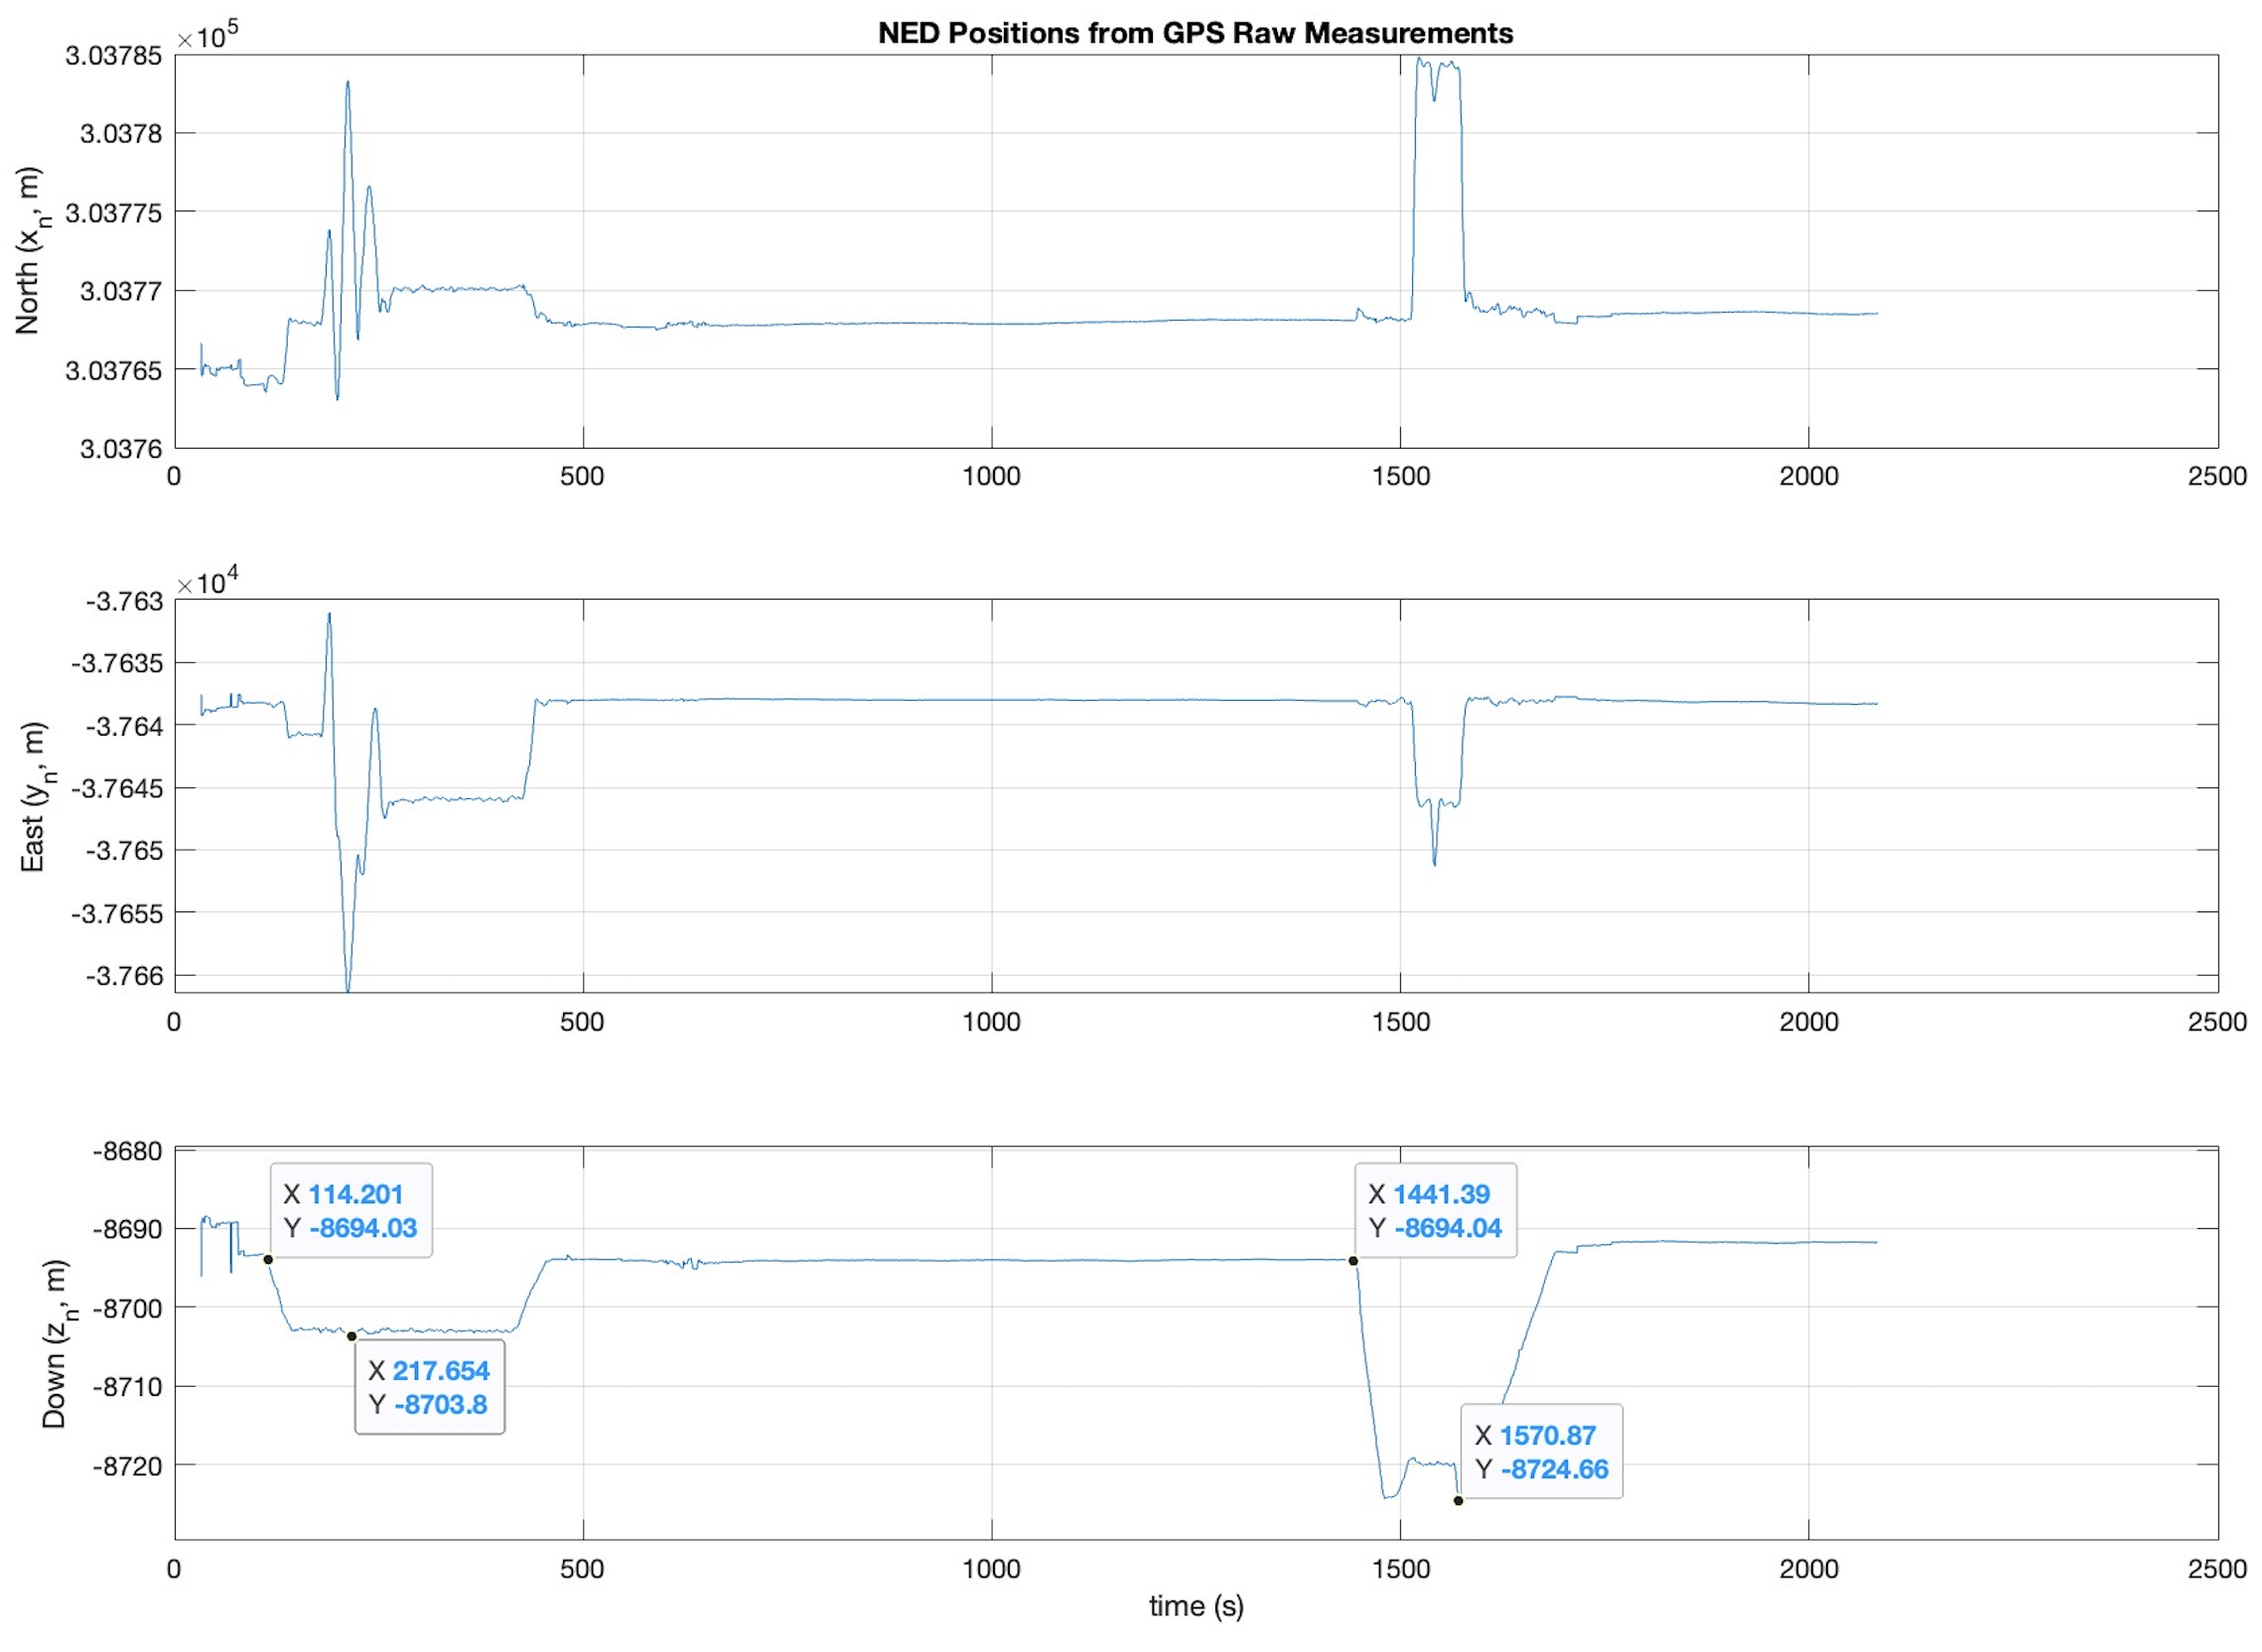
\includegraphics[width=0.8\linewidth, height=0.7\linewidth]{GPS/GPS2NED.png}  
\caption{NED Positions from GPS Raw Measurements}
\label{fig:GPS2NED}
\end{figure}
\\
As the graph in Fig (\ref{fig:GPS2NED}) shows, the UAV takes off twice at the same time frame as the GPS plot. From analyzing the graph, the data shows that during the first UAV take-off and landing, it flies about 10 m (8704 m (max height) - 8694 m ("zero" height)). During the second UAV take-off and landing, it flies approximately 31 m (8725 m (max height) - 8694 m ("zero" height)). The NED positions are validated from the GPS data, showing that the GPS raw measurement to local NED position is completed with great accuracy. We see that the Down ($z_n$ graph is flipped from the GPS Plot, and that is because of the way the axis is defined, but the magnitude of the altitude change for both the GPS plot and the NED positions plot validates the transformation. The code for the transformation from GPS to NED can be found in Fig. (\ref{GPStoNED Matlab Code}). 

\label{GPStoNED Matlab Code}
\begin{lstlisting}
% To obtain local NED from GPS, need to convert Geodetic to ECEF to NED coordinate frame.

% Convert Latitude and Longitude to Radians
lat_rad = deg2rad(lat);
lon_rad = deg2rad(lon);

% Create a function to convert GPS to NED coordinate Frame
function [NED_Coordinates] = GPStoNED(lat_rad, lon_rad, alt)
    % Constants for Earth Ellipsoid to convert from Geodetic to ECEF
    a = 6378137;
    b = 6356752.3142;
    e2 = 1 - (b^2 / a^2);
    % Define initial UAV position as reference position
    lat_0 = lat_rad(1); % Reference Latitude
    lon_0 = lon_rad(1); % Reference Longitude
    alt_0 = alt(1); % Reference Altitude
    % Convert defined intial GPS reference position to ECEF coordinate frame
    [x_e0, y_e0, z_e0] = GPStoECEF(lat_0, lon_0, alt_0, a, e2);
    % Create arrays for NED Coordinates to be stored after iteration
    NED_Coordinates = zeros(length(lat_rad), 3);
    % Loop over all GPS raw measurements and convert each to NED coordinates
    for i = 1:length(lat_rad)
        % Convert GPS raw measurements to ECEF coordinate frame
        [x_e, y_e, z_e] = GPStoECEF(lat_rad(i), lon_rad(i), alt(i), a, e2);
        % Convert ECEF measurements to NED coordinate frame
        [x_n, y_n, z_n] = ECEFtoNED(x_e, y_e, z_e, x_e0, y_e0, z_e0, lat_rad(i), lon_rad(I));
        % Store NED coordinates in created arrays
        NED_Coordinates(i, :) = [x_n, y_n, z_n];
    end
end

% Create a function to convert GPS to ECEF coordinate frame
function [x_e, y_e, z_e] = GPStoECEF(lat, lon, alt, a, e2)
    % Define radius of curvature
    N = a ./ sqrt(1 - e2 .* sin(lat).^2); % Radius of curvature
    % Convert GPS raw measurements to ECEF coordinate frame
    x_e = (N + alt) .* cos(lat) .* cos(lon);
    y_e = (N + alt) .* cos(lat) .* sin(lon);
    z_e = ((1 - e2) .* N + alt) .* sin(lat);
end

% Create a function to convert ECEF to NED coordinate frame
function [x_n, y_n, z_n] = ECEFtoNED(x_e, y_e, z_e, x_e0, y_e0, z_e0, lat, lon)
    % Difference between ECEF current coordinate and ECEF reference point
    dx = x_e - x_e0;
    dy = y_e - y_e0;
    dz = z_e - z_e0;
    % Rotation matrix to go from ECEF to NED coordinate system
    R = [-sin(lat) * cos(lon), -sin(lon) , -cos(lat) * cos(lon) ;
         -sin(lat) * sin(lon), cos(lon)  , -cos(lat) * sin(lon) ;
         cos(lat)            ,     0     , -sin(lat)           ];
    % Calculate NED coordinates
    NED = R' * [dx; dy; dz];
    x_n = NED(1); y_n = NED(2); z_n = NED(3);
end

% Run the NED_Coordinates function to compute a GPS to NED Coordinate
% Transform and substitute into correct naming convention [x_n, y_n, z_n]
[NED_coords] = GPStoNED(lat_rad, lon_rad, alt);
x_n = NED_coords(:,1); y_n = NED_coords(:,2); z_n = NED_coords(:,3);

%% GPS to NED Plot
figure; set(gcf,'numbertitle','off','name','NED Positions from GPS Raw Measurements');  
subplot(3,1,1); plot(t(125:end), x_n(125:end));title('NED Positions from GPS Raw Measurements'); ylabel('North (x_n, m)'); grid on;
subplot(3,1,2); plot(t(125:end), y_n(125:end)); ylabel('East (y_n, m)'); grid on;
subplot(3,1,3); plot(t(125:end), z_n(125:end)); ylabel('Down (z_n, m)'); grid on; xlabel('time (s)');
\end{lstlisting}
\captionof{figure}{MATLAB Code for GPS Raw Measurement to Local NED Positions}
\label{fig:GPS2NEDMatlab}
